\documentclass[aspectratio=169,10pt]{beamer}
\usetheme{Madrid}
\usecolortheme{seahorse}

\usepackage[utf8]{inputenc}
\usepackage{amsmath}
\usepackage{amssymb}
\usepackage{amsfonts}
\usepackage{mathtools}
\usepackage{listings}
\usepackage{xcolor}
\usepackage{graphicx}

% Code listing style
\lstset{
    basicstyle=\ttfamily\tiny,
    commentstyle=\color{green!50!black}\itshape,
    keywordstyle=\color{blue}\bfseries,
    stringstyle=\color{red},
    numbers=left,
    numberstyle=\tiny\color{gray},
    frame=single,
    breaklines=true,
    tabsize=2,
    language=Python
}

\setbeamertemplate{footline}[frame number]
\graphicspath{{figures/}}

\title{Chapter 5g: Fixed Point Theorems in Banach Algebra and Lattice-Theoretic Structures}
\subtitle{P-Lipschitzian Maps, Lattice Fixed Points, and Cascading Nonexpansive Maps}
\author{From Pathak's \textit{An Introduction to Nonlinear Analysis and Fixed Point Theory}}
\date{}

\begin{document}

\frame{\titlepage}

\begin{frame}{Outline}
  \tableofcontents
\end{frame}

% ============================================================================
\section{Overview}

\begin{frame}{Chapter Overview}
  \begin{itemize}
    \item \textbf{Section 5.8:} Fixed Point Theorems in Banach Algebra
      \begin{itemize}
        \item P-Lipschitzian Maps (Definition 5.94)
        \item Fixed point existence for multiple operators
      \end{itemize}

    \vspace{0.3cm}

    \item \textbf{Section 5.9:} Lattice-Theoretic Fixed Point Theorems
      \begin{itemize}
        \item Tarski's fixed point theorem
        \item Increasing functions on lattices
      \end{itemize}

    \vspace{0.3cm}

    \item \textbf{Section 5.9.1:} Reflexivity and Perturbed Fixed Point Property
      \begin{itemize}
        \item James's distortion theorems
        \item Cascading nonexpansive maps
      \end{itemize}
  \end{itemize}
\end{frame}

% ============================================================================
\section{Fixed Point Theorems in Banach Algebra}

\begin{frame}{Mapping Classification}
  \centering
  
\includegraphics[width=0.85\textwidth]{mapping_hierarchy.pdf}
\end{frame}

\begin{frame}{Definition 5.94: P-Lipschitzian Maps}
  \begin{definition}
    A mapping $T: X \to X$ on a Banach space $X$ is called \textbf{P-Lipschitzian}
    if there exists a nondecreasing function $\phi: \mathbb{R}^+ \to \mathbb{R}^+$ such that
    \[\|Tx - Ty\| \leq \phi(\|x - y\|), \quad \forall x, y \in X\]
  \end{definition}

  \vspace{0.3cm}

  \textbf{Key Observations:}
  \begin{itemize}
    \item Every D-Lipschitzian mapping is P-Lipschitzian
    \item The converse is \textit{not} true in general
    \item More general than classical contractions
  \end{itemize}
\end{frame}

\begin{frame}{Theorem 5.183: Operator Equation with P-Lipschitzian Operators}
  \begin{theorem}
    Let $S$ be a closed, convex and bounded subset of a Banach algebra $X$, and
    let $A, C: X \to X$ and $B: S \to X$ be three operators such that
    \begin{enumerate}
      \item[(a)] $A$ and $C$ are P-Lipschitzian with P functions $\phi_A$ and $\phi_C$;
      \item[(b)] $B$ is completely continuous; and
      \item[(c)] $x = AxBy + Cx \Rightarrow x \in S$, $\forall y \in S$.
    \end{enumerate}

    Then $AxBx + Cx = x$ has a solution whenever
    $M\phi_A(r) + \phi_C(r) < r$, $r > 0$, where $M = \|B(S)\|$.
  \end{theorem}
\end{frame}

\begin{frame}{Theorems 5.184 and 5.185: D-Lipschitzian Variants}
  \begin{theorem}[Theorem 5.184]
    Let $S$ be a closed, convex and bounded subset of a Banach algebra $X$, and
    let $A: X \to X$ and $B: S \to X$ be two operators such that
    \begin{enumerate}
      \item[(a)] $A$ is D-Lipschitzian;
      \item[(b)] $(I/A)^{-1}$ exists on $B(S)$; and
      \item[(c)] $x = AxBy \Rightarrow x \in S$, $\forall y \in S$.
    \end{enumerate}

    Then $AxBx = x$ has a solution whenever $M\phi(r) < r$, where $M = \|B(S)\|$.
  \end{theorem}
\end{frame}

\begin{frame}{Proposition 5.14: Sufficient Condition}
  \begin{theorem}
    Let $S = \{y \in X : \|y\| \leq r\}$ be a closed ball in Banach algebra $X$.
    Let $A, C: X \to X$ and $B: S \to S$ be operators satisfying hypothesis (a)--(b)
    of Theorem 5.177. If
    \[\left\|\left(\frac{I - C}{A}\right) x\right\| \leq \|x\|\]
    for all $x \in X$, then $x \in S$.
  \end{theorem}
\end{frame}

\begin{frame}{Visualization: Fixed Point Iteration}
  \centering
  
\includegraphics[width=0.95\textwidth]{fixed_point_iteration.pdf}
\end{frame}

% ============================================================================
\section{Lattice-Theoretic Fixed Point Theorems}

\begin{frame}{Banach Lattice Structure}
  \centering
  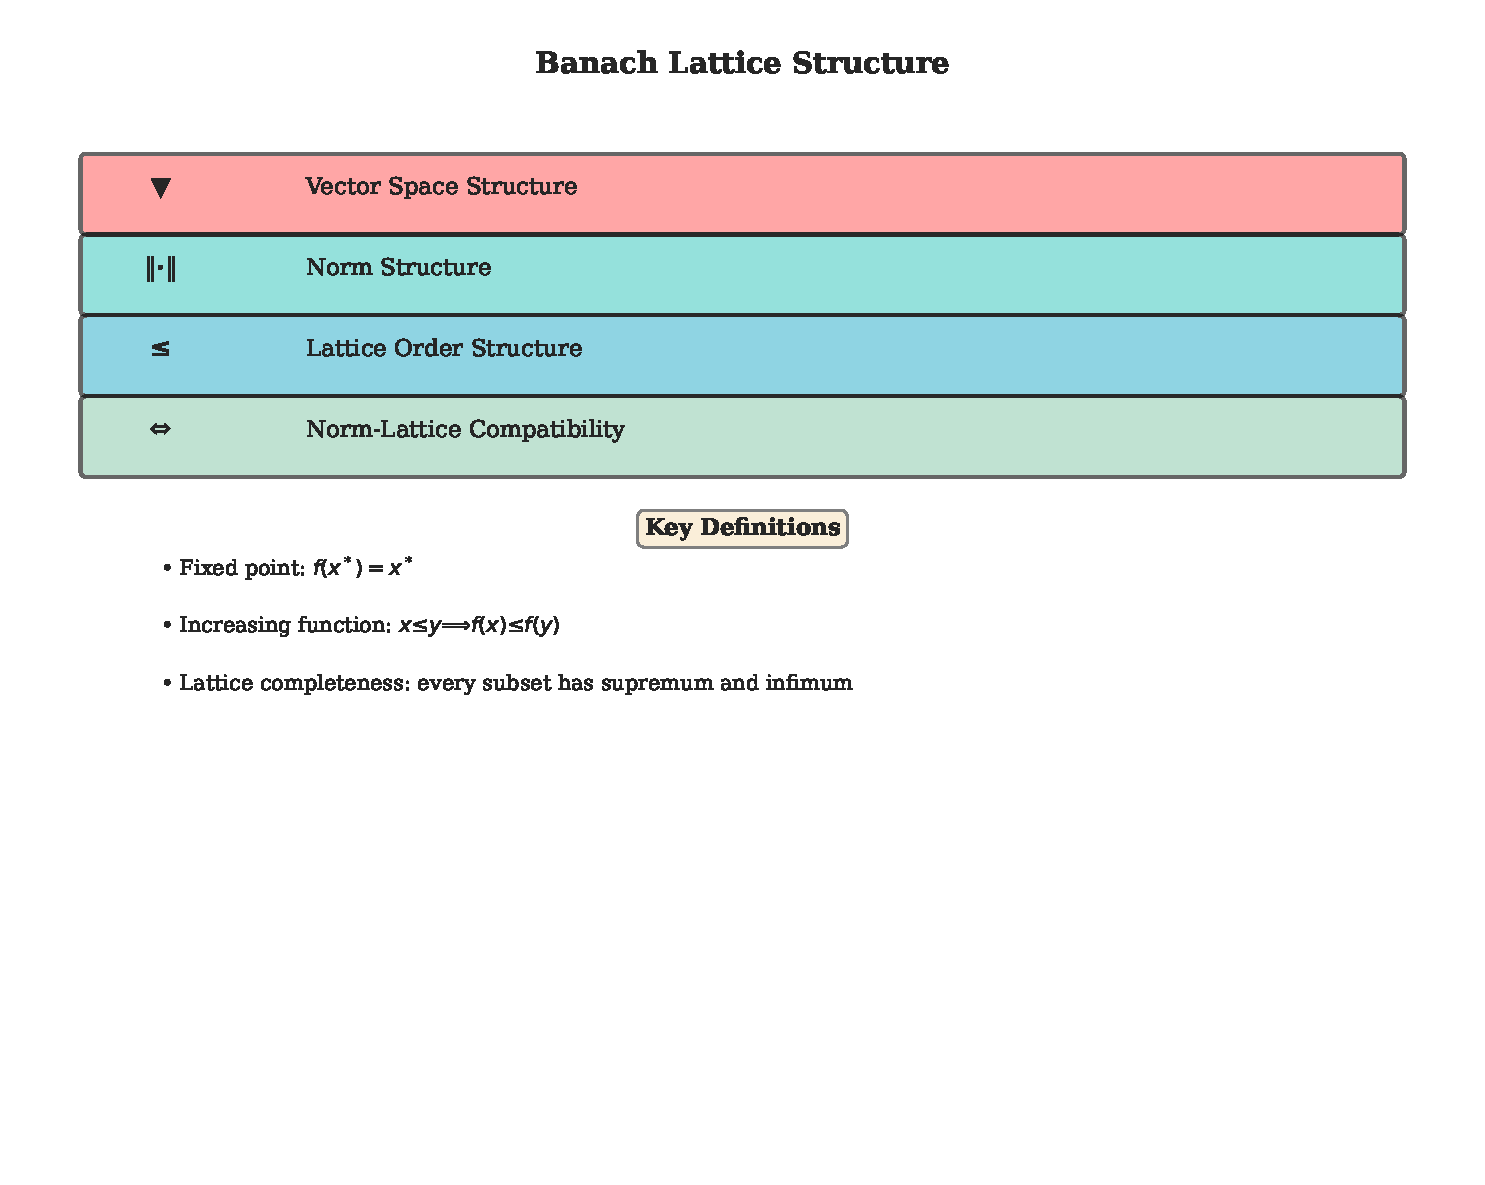
\includegraphics[width=0.85\textwidth]{banach_lattice_structure.pdf}
\end{frame}

\begin{frame}{Theorem 5.186: Tarski's Fixed Point Theorem}
  \begin{theorem}[Tarski]
    Let $\mathfrak{A} = (A, \leq)$ be a complete lattice and $f$ be an increasing function on $A$ to $A$.
    Let $P$ be the set of all fixed points of $f$.

    Then $P$ is not empty, and $(P, \leq)$ is a complete lattice; in particular,
    \[\bigcup P = \bigcup \{x \in A : f(x) \geq x\} \in P\]
    and
    \[\bigcap P = \bigcap \{x \in A : f(x) \leq x\} \in P.\]
  \end{theorem}

  \vspace{0.2cm}

  \textbf{Key Ideas:}
  \begin{itemize}
    \item No contractivity assumption!
    \item Applies to arbitrary increasing functions
    \item Fixed points form a complete lattice
  \end{itemize}
\end{frame}

\begin{frame}{Theorem 5.187: Generalized Lattice-Theoretic Result}
  \begin{theorem}
    Let $\mathfrak{A} = (A, \leq)$ be a complete lattice and $F$ be a commutative set of
    increasing functions on $A$ to $A$. Let $P$ be the set of all common fixed points
    of all functions $f \in F$.

    Then $P$ is not empty and $(P, \leq)$ is a complete lattice.
  \end{theorem}

  \vspace{0.3cm}

  \textbf{Extension:} Allows multiple \textit{commuting} functions; their common
  fixed points form a complete lattice.
\end{frame}

\begin{frame}{Theorem Comparison}
  \centering
  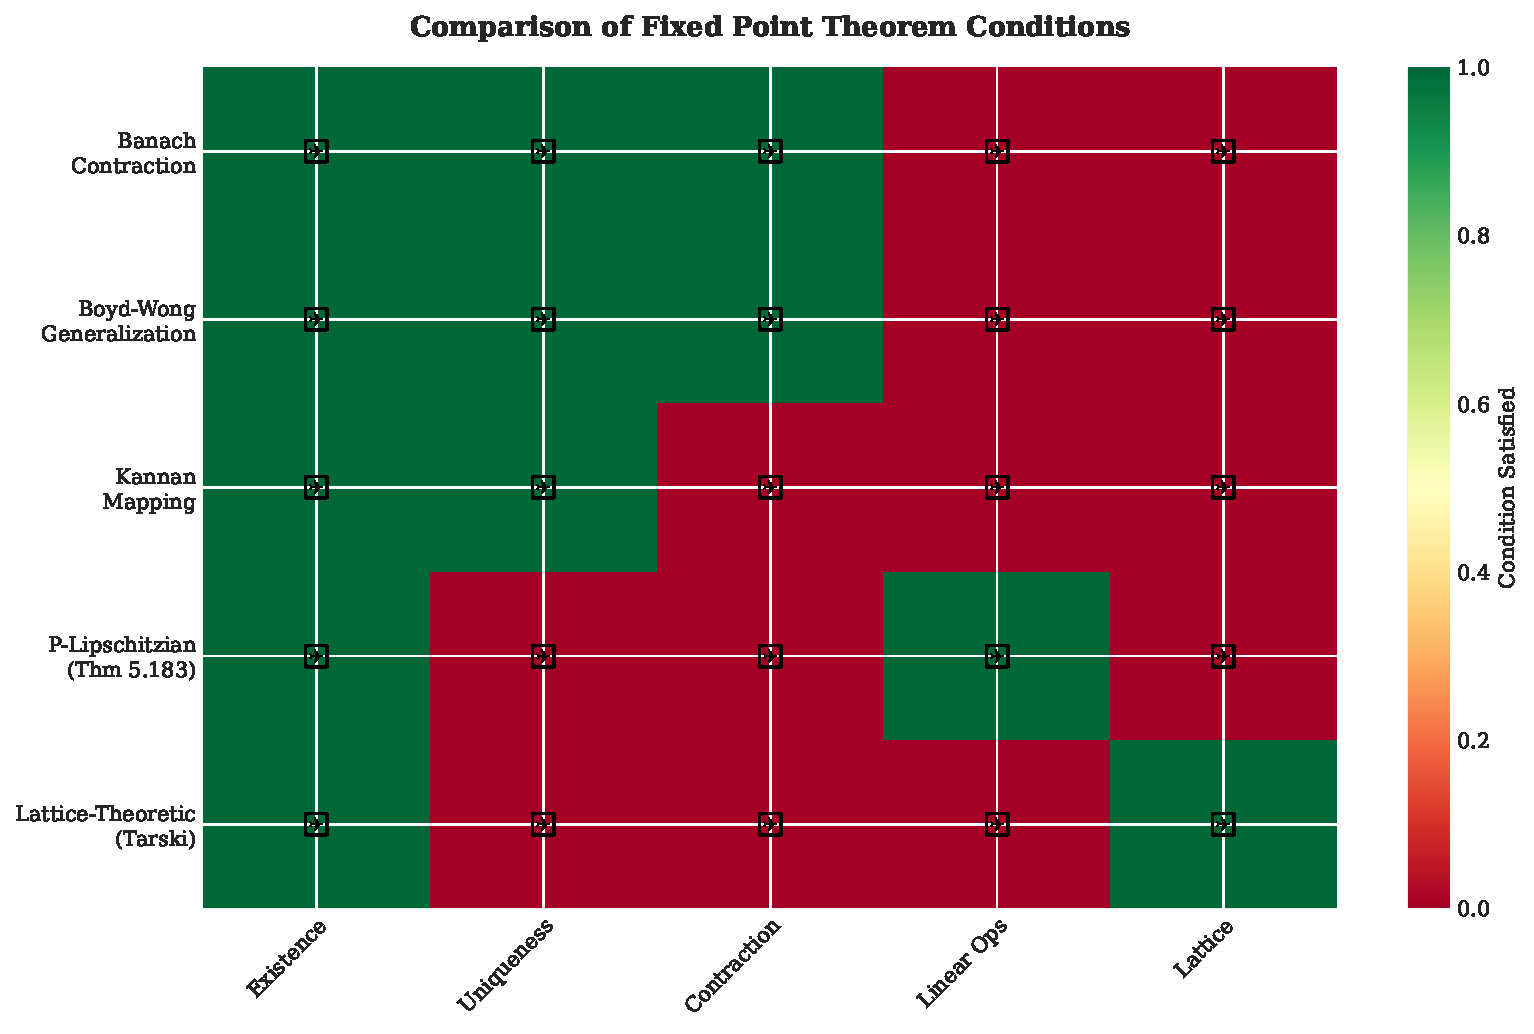
\includegraphics[width=1.0\textwidth]{theorem_comparison.pdf}
\end{frame}

% ============================================================================
\section{Reflexivity and Cascading Nonexpansive Maps}

\begin{frame}{Cascading Nonexpansive Mappings}
  \begin{definition}
    A mapping $T: C \to C$ on bounded, closed and convex subset $C$ is
    \textbf{cascading nonexpansive} if there exists $(k_n) \in [1, \infty)$ with
    $k_n \to 1$ such that for all $n \in \mathbb{N}$ and $x, y \in C_n$,
    \[\|Tx - Ty\| \leq k_n \|x - y\|\]
    where $C_0 := C$ and $C_n := \overline{co}(T(C_{n-1})) \subseteq C_{n-1}$.
  \end{definition}

  \vspace{0.2cm}

  \textbf{Key Properties:}
  \begin{itemize}
    \item Norm-to-norm continuous
    \item Generalizes nonexpansive maps
    \item Arises naturally in $\ell_1$ and $c_0$ spaces
  \end{itemize}
\end{frame}

\begin{frame}{James's Distortion Theorems}
  \begin{theorem}[James's Distortion Theorem for $\ell_1$]
    A Banach space $X$ contains an isomorphic copy of $\ell_1$ iff for every
    null sequence $(\varepsilon_n)$ in $(0, 1)$, there exists $(x_n) \subseteq X$ such that
    \[(1 - \varepsilon_n) \sum_{n=k}^{\infty} |t_n| \leq \left\|\sum_{n=k}^{\infty} t_n x_n\right\|
    \leq \sum_{n=k}^{\infty} |t_n|\]
    for all $(t_n) \in \ell_1$ and $k \in \mathbb{N}$.
  \end{theorem}
\end{frame}

\begin{frame}{Theorem 5.188: Fixed Point Freeness}
  \begin{theorem}[Theorem 5.188]
    Let $(X, \|\cdot\|)$ be a Banach space containing an isomorphic copy of
    $\ell_1$ or $c_0$. Then there exists a bounded, closed and convex set $C \subseteq X$
    and an affine cascading nonexpansive mapping $T: C \to C$ that is
    \textbf{fixed point free}.
  \end{theorem}

  \vspace{0.3cm}

  \textbf{Implication:} Non-reflexive spaces may fail fixed point property!
\end{frame}

\begin{frame}{Theorems 5.189 and 5.190: Reflexivity Characterization}
  \begin{theorem}[Theorem 5.189]
    Let $(X, \|\cdot\|)$ be a reflexive Banach space. Then there exists an equivalent
    norm $\|\cdot\|_-$ on $X$ such that for every bounded, closed and convex subset
    $C \subseteq X$, every $\|\cdot\|_-$-cascading nonexpansive mapping $T: C \to C$
    has a fixed point in $C$.
  \end{theorem}

  \vspace{0.3cm}

  \begin{theorem}[Theorem 5.190]
    For a Banach lattice (or space with unconditional basis, or operator ideal),
    reflexivity is equivalent to the fixed point property for cascading nonexpansive maps.
  \end{theorem}
\end{frame}

\begin{frame}{Lipschitz Constant Effect on Convergence}
  \centering
  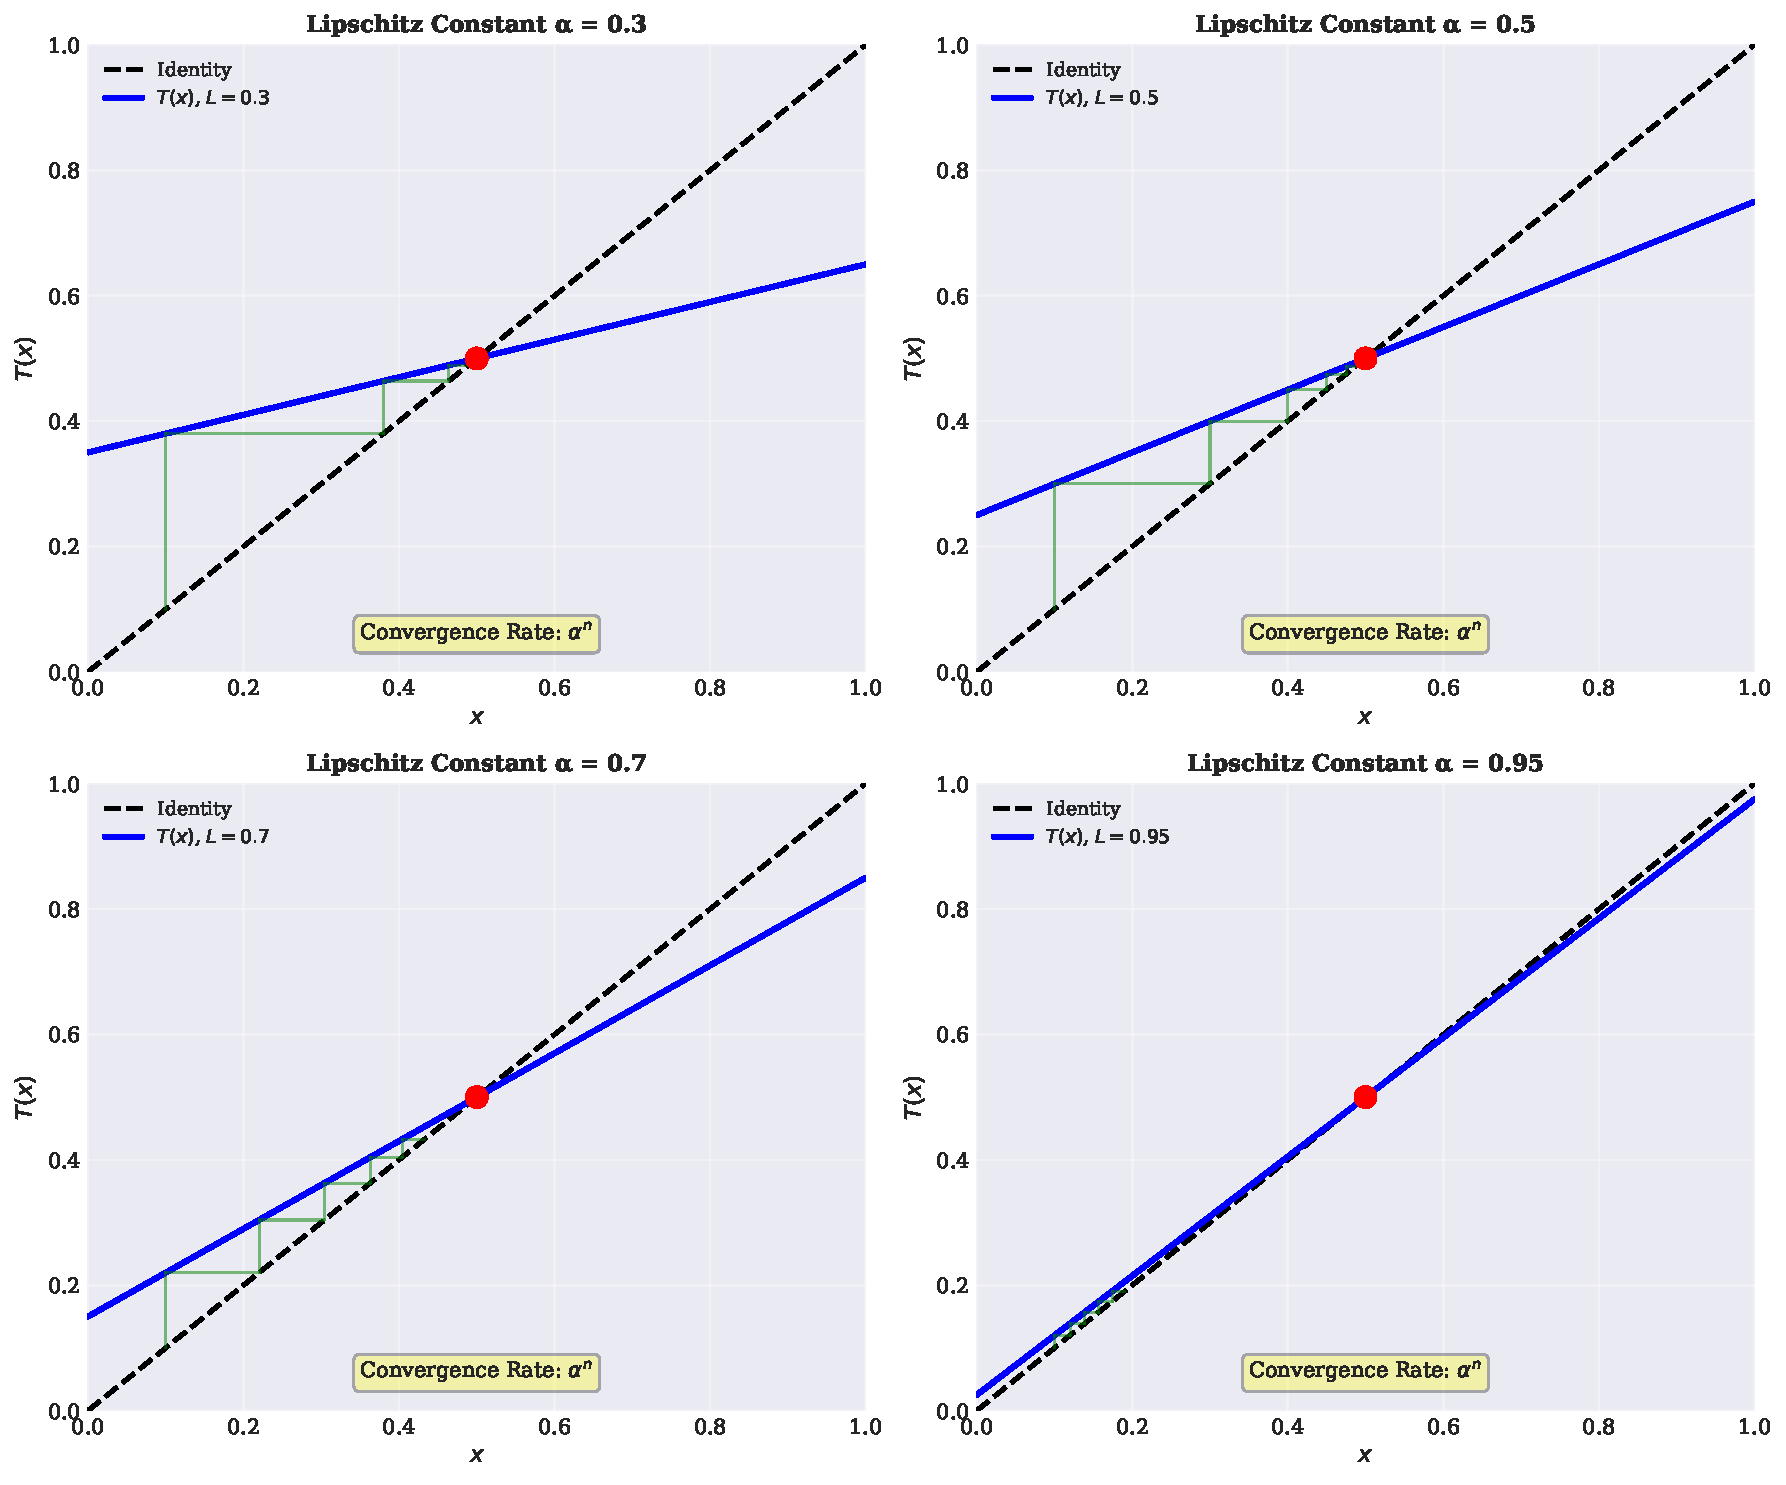
\includegraphics[width=0.95\textwidth]{lipschitz_convergence.pdf}
\end{frame}

% ============================================================================
\section{Applications and Summary}

\begin{frame}{Numerical Example}
  \centering
  
\includegraphics[width=0.95\textwidth]{numerical_example.pdf}
\end{frame}

\begin{frame}{Key Applications}
  \begin{itemize}
    \item \textbf{Operator Equations:} Solving $AxBx + Cx = x$
      in nonlinear systems

    \vspace{0.2cm}

    \item \textbf{Lattice Optimization:} Finding extremal fixed points
      in order-theoretic structures

    \vspace{0.2cm}

    \item \textbf{Banach Space Geometry:} Understanding spaces via
      fixed point properties

    \vspace{0.2cm}

    \item \textbf{Differential and Integral Equations:} Existence and uniqueness
      of solutions with special structure

    \vspace{0.2cm}

    \item \textbf{Iterative Methods:} Design and convergence analysis of
      numerical schemes
  \end{itemize}
\end{frame}

\begin{frame}{Important Distinctions}
  \begin{itemize}
    \item \textbf{Contraction Mappings}
      \begin{itemize}
        \item Unique fixed point, exponential convergence
      \end{itemize}

    \vspace{0.2cm}

    \item \textbf{P-Lipschitzian Maps}
      \begin{itemize}
        \item General function condition, applies to multiple operators
      \end{itemize}

    \vspace{0.2cm}

    \item \textbf{Nonexpansive Maps}
      \begin{itemize}
        \item Requires geometric conditions, more general setting
      \end{itemize}

    \vspace{0.2cm}

    \item \textbf{Lattice-Theoretic}
      \begin{itemize}
        \item Guaranteed existence, no metric required
      \end{itemize}
  \end{itemize}
\end{frame}

\begin{frame}{Key Theorems Summary}
  \begin{itemize}
    \item \textbf{Theorem 5.183--5.185:} P-Lipschitzian and D-Lipschitzian operators
      in Banach algebras with existence conditions

    \item \textbf{Theorem 5.186--5.187:} Tarski's lattice-theoretic theorems with
      no contractivity assumptions

    \item \textbf{Theorems 5.188--5.190:} Reflexivity characterization via
      cascading nonexpansive maps in Banach lattices

    \item \textbf{James's Distortion Theorems:} Characterization of $\ell_1$ and
      $c_0$ in Banach spaces
  \end{itemize}
\end{frame}

\begin{frame}
  \centering
  \vspace{1cm}

  {\Huge \textbf{Questions?}}

  \vspace{1cm}

  {\normalsize Chapter 5g: Fixed Point Theorems in Banach Algebra and Lattice Structures}
\end{frame}

\end{document}
